%%================================================
%% Filename: chap01.tex
%% Encoding: UTF-8
%% Author: Yuan Xiaoshuai - yxshuai@gmail.com
%% Created: 2012-04-27 15:05
%% Last modified: 2016-08-28 21:07
%%================================================
\chapter{绪论}
\label{cha:overview}

\section{研究背景及意义}

近年来随着普及和使用率持续增长,互联网已然成为全球信息交流、经济发展和社会融合的关键基础
设施,在现代社会中有着不可或缺的地位。中国互联网络信息中心(China Internet 
Network Information Center,CNNIC)第 48 次《中国互联网络发展状况统计报告》显
示\cite{cnnic2021}, 截至 2021 年 6 月,我国所使用的 IPv4 地址总数接近 4 亿,IPv6 地址总数
超过了 6万。根据ITU(International Telecommunication Union)的《事实与数据2023报告》显示\cite{itu2023},截止2022年12月,全球共有网民数49.5亿;
截至2023年,全球约有67\%的人口,即大约54亿人正在使用互联网。图~\ref{fig:individula_using_internet}~显
示了近几年全球网民数量及占比的变化。这些数据表明当前网络规模在急剧扩大,网络多样性也在逐渐增加。
\begin{figure}[htbp]
    \centering
    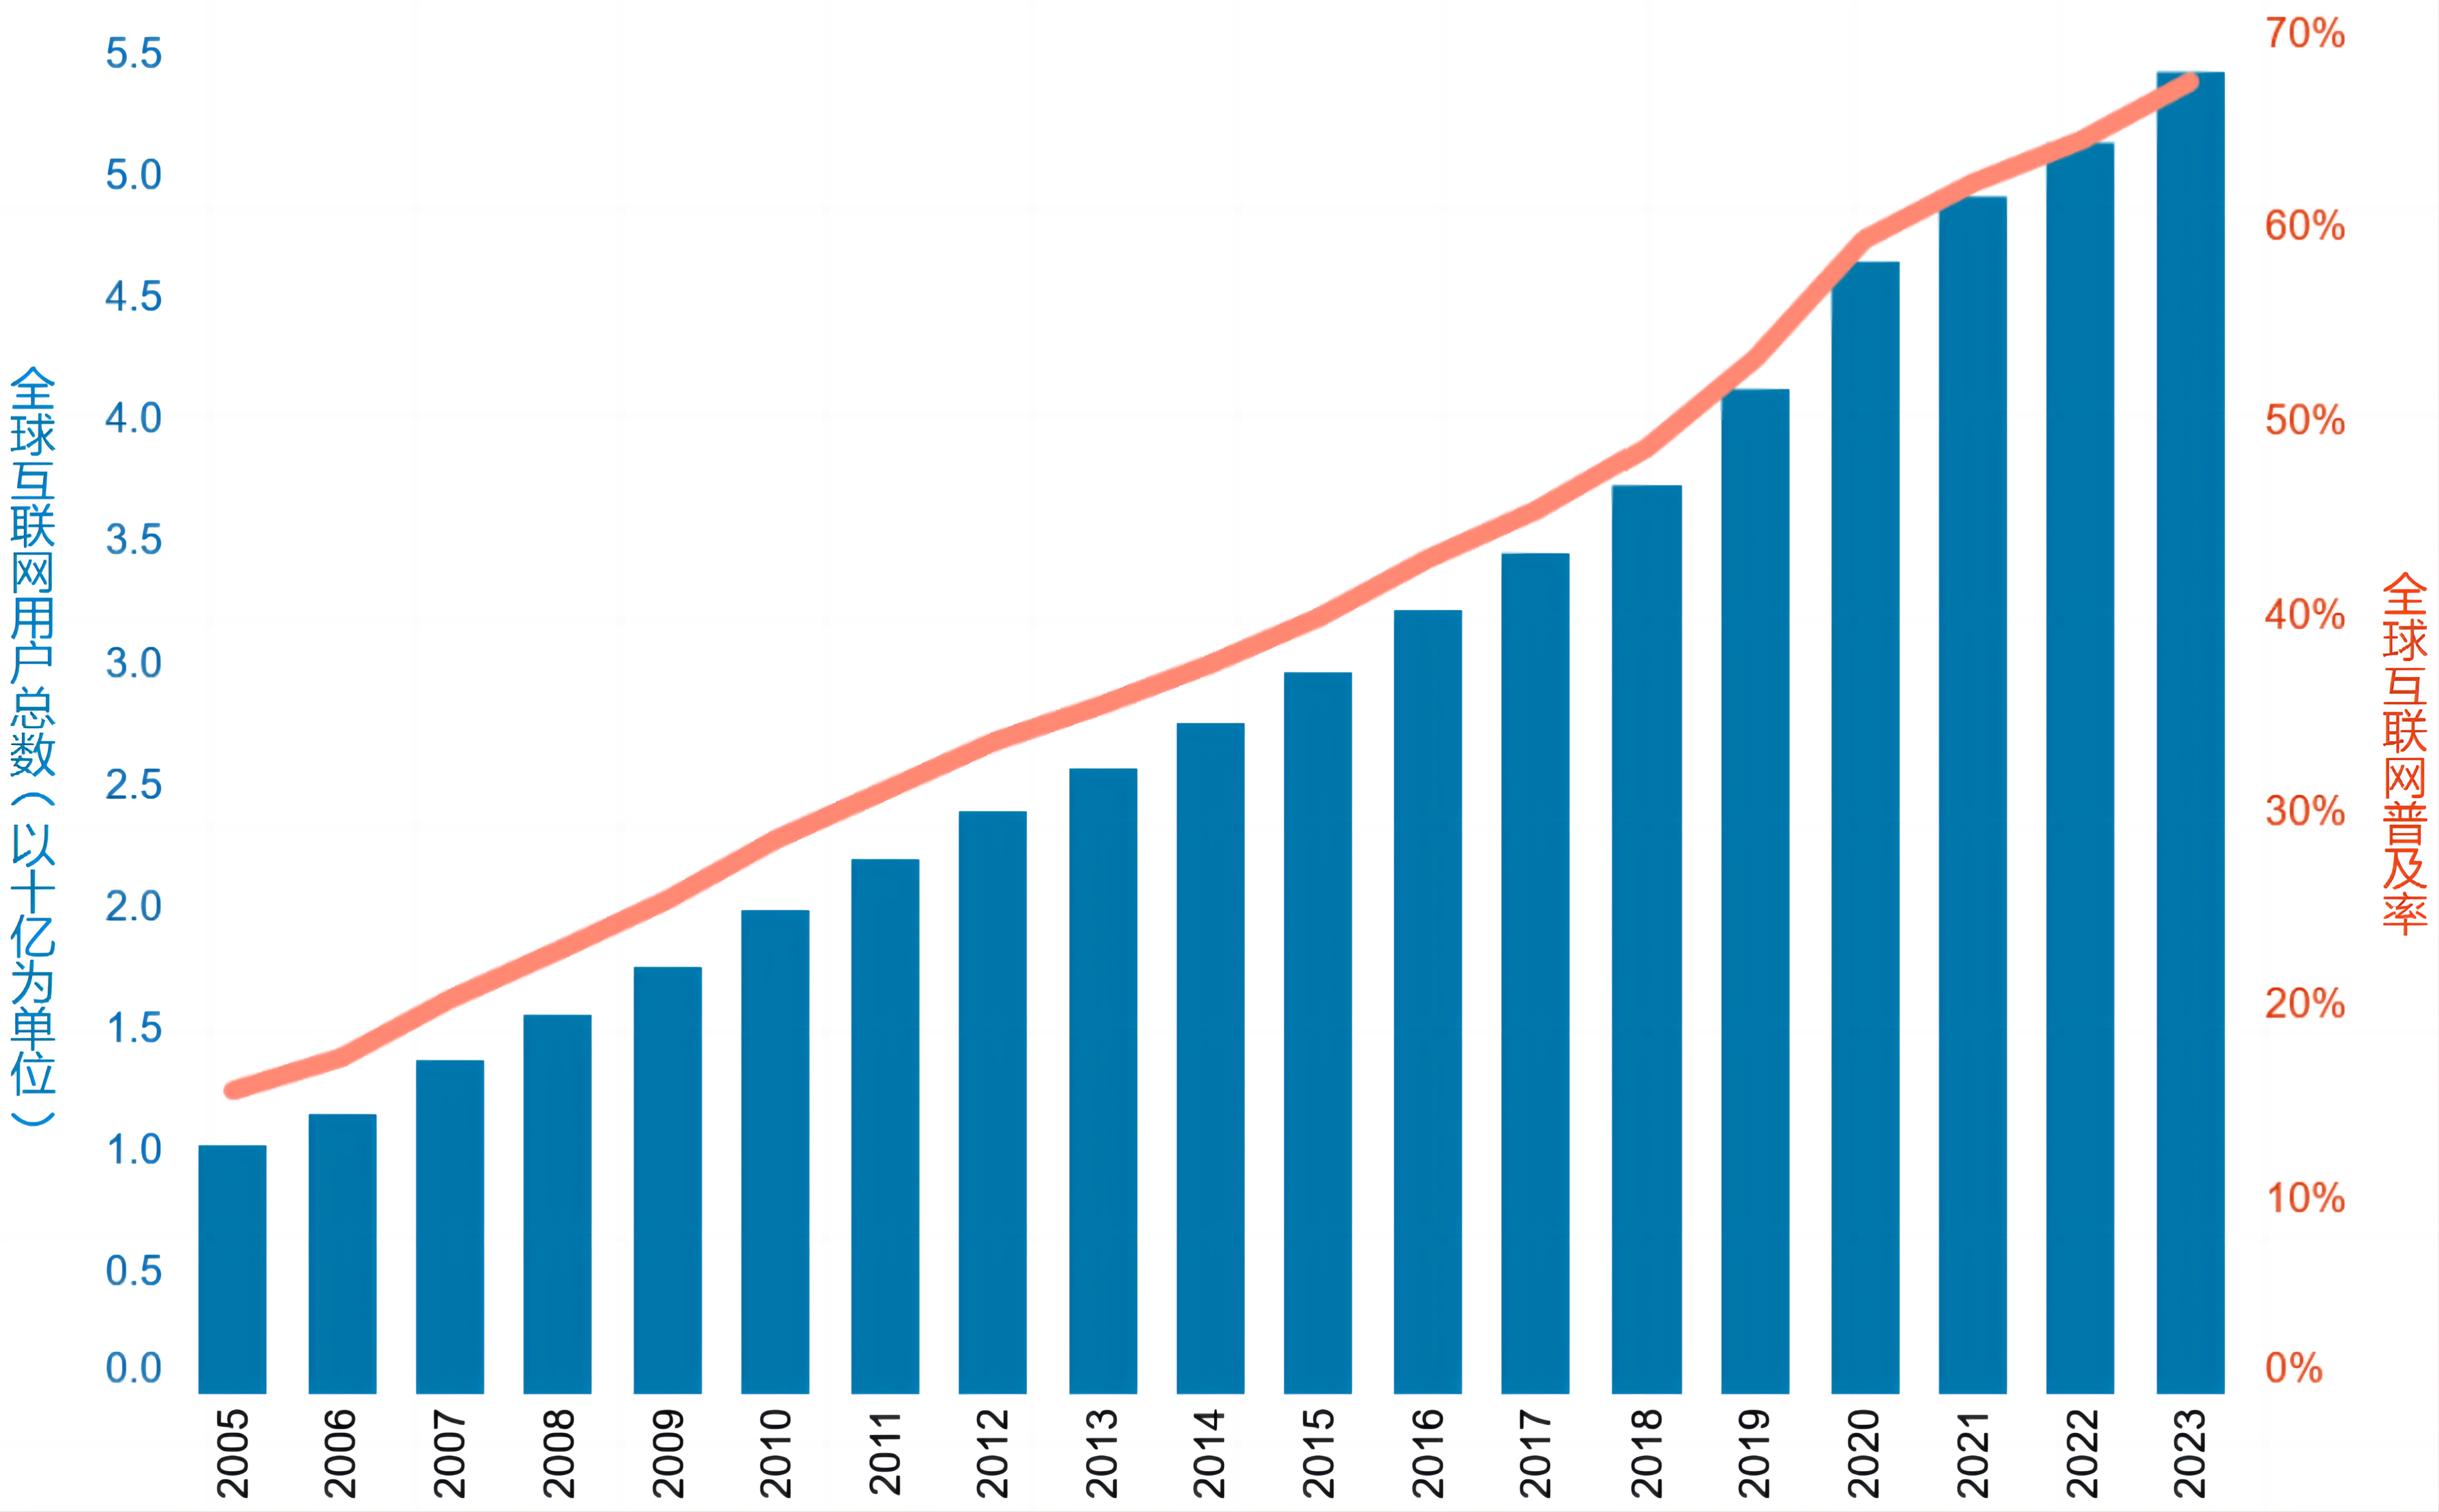
\includegraphics[width = 0.8\textwidth]{individula_using_internet.png}
    \caption{全球网民数量及普及率变化\cite{fig-itu2023}}
    \label{fig:individula_using_internet}
\end{figure} 


尽管互联网规模的扩大为社会经济和科技进步提供了强大的推动力,并为全人类带来了前所未有的便利,但它却是一把双刃剑,伴
随而来的是一系列隐患和威胁,对我们的生活和安全、甚至是国家的稳定都构成了严重的威胁。
2021年,未知攻击者窃取GoDaddy源代码并在其服务器上安装恶意软件,影响了120万Managed WordPress客户的个人信息。
2022年12月,PayPal遭到凭证填充攻击,攻击者通过尝试使用从其他网站数据泄露中获得的用户名和密码对,成功访问了34,942个账户。
2023年5月末,由Clop勒索软件团伙发起了MOVEit攻击。这次攻击利用了Progress MOVEit文件传输工具的关键漏洞,影响了
2,667个组织和近8400万个人,MGM也因此事件估计损失了1亿美元​。此事件被认为是2023
年范围最广的攻击之一,也是近年来最大的数据盗窃事件之一。图~\ref{fig:daily_web_application_attacks}~展示了Akamai关于2022年
与2023年网络攻击每日统计数量。
这些数据表明,随着互联网的广泛普及,网络攻击者日益有组织、专业化,新型网络攻击层出不穷,其特性日益高维、复杂,难以识别。


% 这些原因最终将导致网络攻击变得更加具有破坏力且难以被识别,网络安全形式将变得比以往更加严峻。

\begin{figure}[htbp]
  \centering
  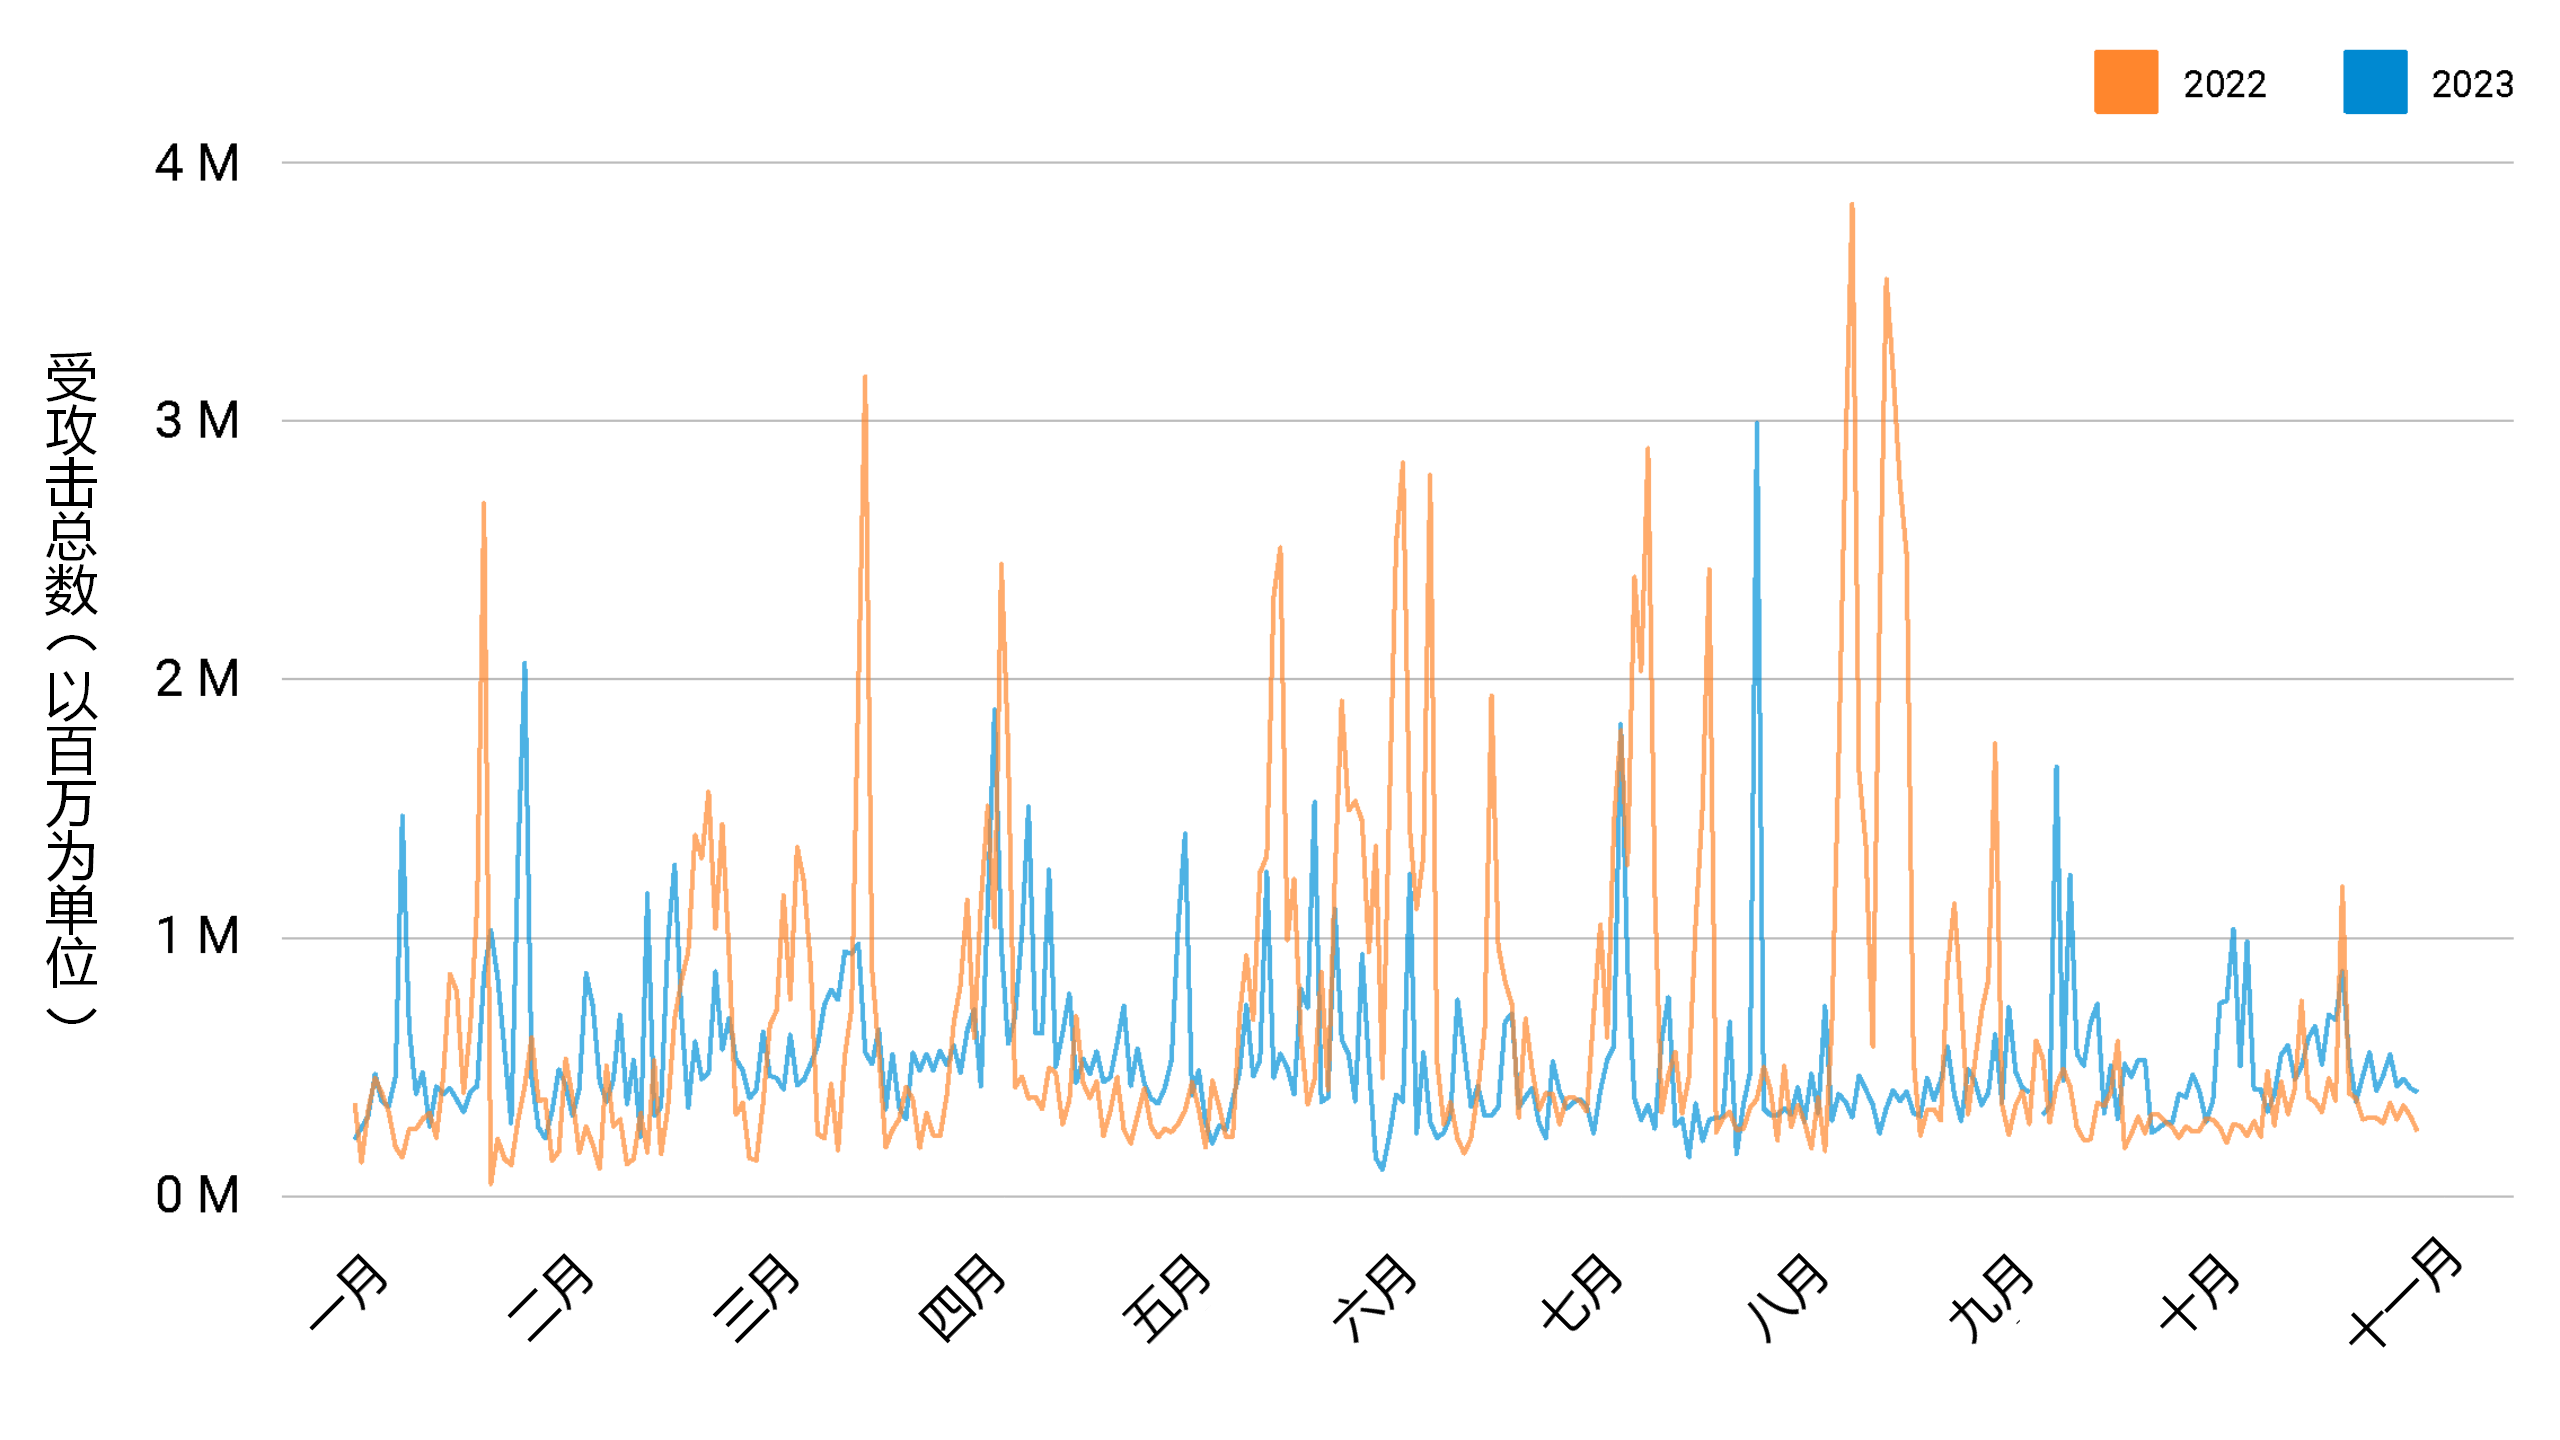
\includegraphics[width = 0.8\textwidth]{daily_web_application_attacks.png}
  \caption{2022年与2023年网络攻击每日统计数量\cite{akamai}}
  \label{fig:daily_web_application_attacks}
\end{figure}

% 网络攻击如此猖獗的原因除了互联网的普及以及网络攻击人员组织化、专业化这些因素之外,
% 网络本身的设计缺陷同样也是一个重要的因素。由于Internet数据传输采用无连接的逐跳转发模式,使
% 网络节点之间的数据包在网络层传输时仅以目的IP进行寻址转发,由此可能导致网络中的恶意节点伪造数据包中源端的IP地址以欺骗目的节点进行非
% 法通信窃取目的端用户的相关信息,导致了基于源地址欺骗类型的网络攻击行为的出现,如MITM、
% 洪泛攻击、反射式攻击、DoS/DDoS攻击等\cite{zhen2022}。攻击数据包中的源地址字段一旦被伪造,就使得识别数据包的来源变得复杂。互联网的无状态
% 特性几乎使得识别攻击的真正来源变得不切实际\cite{singh2016}。这一问题除了导致网络攻击难以
% 被根除之外,还可能引发其他恶意行为,例如恶意用户冒充目标用户的身份,触发运营商或其他服务提供
% 商的管理规则,进而危害目标主机的声誉和利益。解决这个问题对于网络生态系统的安全至关重要。\par

% 随着网络攻击的不断演进,研究者们也在不断采取新的措施来应对这些挑战。从
% 早期的防火墙和反病毒软件的部署,到现在的机器学习和人工智能技术的应用,
% 网络安全领域经历了快速的发展。在20世纪90年代,随着互联网的普及,网络攻击开始成为一个严重的问题。研究    借记卡  
% 者们首先采取的措施是开发和部署防火墙\cite{Ioannidis2000DistributedFirewall}
% 和反病毒软件\cite{Cohen1983},这些基本工具在当时对抵御攻击起到了一定
% 的作用。进入21世纪,随着攻击手段的不断升级,单纯依靠防火墙和反病毒软件已经无法满
% 足防御需要。因此,研究者开始探索新的防御技术。2000年代中期,随着云计算的兴起,
% 研究者开始开发基于云的安全服务\cite{Hashizume2013AnalysisSecurityCloud},
% 这些服务可以提供更灵活、更强大的防御能力。到了2010年代,随着大数据和人工智能技术的发展,研究者开始利用这些技术来提升网络安全。
% 通过分析海量的网络数据,机器学习算法可以识别出复杂的攻击模式,提前预警可能的安全威胁。\par



面对当前日益严峻的网络安全形势,有效识别和应对不断涌现且特征维度持续攀升的新型网络攻击,对于确保网络安全具有不可估量的重要意义。
虽然现有的网络攻击检测技术相比过去已有显著进步,但面对复杂多变的网络环境,仍存在诸多挑战。
首先,海量流量数据日益高维化、复杂化,其多维特征使得单一的检测维度难以全面捕捉。
因此,网络攻击检测模型的准确率受到限制。
若能从多个维度综合分析流量数据,必将进一步提升检测的准确度。
其次,当前的异常流量检测模型大多依赖于静态数据集,难以适应网络环境的动态变化。
特别是随着新型网络攻击的不断涌现,模型的检测性能往往大幅下降。
因此,设计一个既能保持高检测准确率又能灵活应对新型攻击的模型成为迫切需求。
最后,现有的异常流量检测模型主要停留在被动检测层面,缺乏主动处理能力和源头解决方案。
例如,在面对DDoS攻击时,若模型仅依赖源IP地址过滤异常流量,一旦攻击者频繁更换僵尸节点的IP地址,模型将不堪重负,甚至崩溃。
因此,为模型设计一套有效的防护机制,从源头上解决异常流量问题,成为当务之急。
% 虽然这些技术在互联网发展5的各个环节对网络安全的防护都具备一定的积极作用,
% 但这些方法却没有考虑到TCP/IP协议本身存在的缺陷,即:网络在运行过程中通常不会对
% 数据包源地址的真实性进行验证。这意味着,即便现有算法能够准确地识别并阻止网络攻击,然而,
% 一旦攻击者变更其源IP地址,系统就必须重新进行攻击检测。当攻击者发送大量带有虚假IP地址的
% 数据包时,防护系统的表现效果将大打折扣。为了应对这个问题,IP回溯技术应运而生。
% 该技术通过受害者主机与多个网络设备的协作,利用网络运行所产生的信息,对攻击路径进行重构,
% 从而揭露攻击源的实际位置。\par 

% 在众多的网络回溯方法中,概率包标记法以其简单、灵活、易于部署及无需人工参与的特点脱颖而出,同时它还支持事后分析,为网络安全领域提供了重要的技术支持。
% 然而,概率包标记法在速度方面存在明显的短板,路径重构过程中需要收集大量的数据包,这无疑增加了时间成本和处理复杂性。
% 针对概率包标记法速度慢的问题,本文提出一种基于路由器接口号分组的概率包标记法。
% 该方法利用路由器接口号作为标记信息,提高了标记空间的利用率。
% 通过该方法,单个数据包便能携带一组标记信息,显著减少所需收集的数据包数量,进而大幅提升路径重构的速度与效率。\par

% 此外,当前的网络方案多依赖于静态的数据集,这在动态变化的网络环境中显然是不够的。
% 为了应对这一挑战,本文还提出一个基于多模态特征融合的增量学习方案。
% 该方案结合残差网络与双向门控循环单元的优势,充分挖掘网络数据的时空特征,并通过增量学习的方式,不断适应网络环境的变化。
% 这种方案不仅提高了检测的准确性,还增强了模型的适应性,为动态网络环境下的网络安全提供了有力保障。\par


% 因此,本文基于这一愿景,设计了一个网络攻击检测及溯源系统,
% 该系统能够在检测到异常流量时,精确地确定攻击主机的实际地址。

\section{国内外研究现状}
% 在本小节中,我们将会对网络溯源相关的研究现状进行分析。
% 一般情况下,溯源只有在系统检测到攻击时才会进行网络溯源。
% 因此本文的工作将会围绕网络溯源和网络攻击检测这两个研究方向共同进行。
% 此处的研究现状也会围绕这两个研究方向分别展开叙述。

% \subsection{网络溯源研究现状}
% IP追踪方案可以根据用于收集追踪信息的底层方法进行分类。这些方法在部署策略、存储需求、
% 信息收集算法等方面可能有所不同。下面给出了几种常见的溯源方法\cite{singh2016}。
% 这几种方法的性能表较如图~\ref{tb:compare_approch}~所示。

% \textbf{链路测试法:}链路测试会对所有上游链路进行递归的分析,直到到达源点为止,以确定传递攻击数据包的链路。
% 从最接近受害者的路由器开始,直到攻击者的源路由器。图~\ref{fig:linktest}~展示了此方法的基本原理。2000年,Burch提出了基于这一
% 原则的第一个IP回溯方案\cite{Burch2000Tracing}。随后是一些基于链接测试的回溯方案
% \cite{HamediHamzehkolaie2012DOSTraceback,ShiYang2005DDoSDefense,
% ThingSlomanDulay2008DDoSDetection}。
% 链路测试方案有两种:输入调试和控制洪水。

% \begin{figure}[htbp]
%   \centering
%   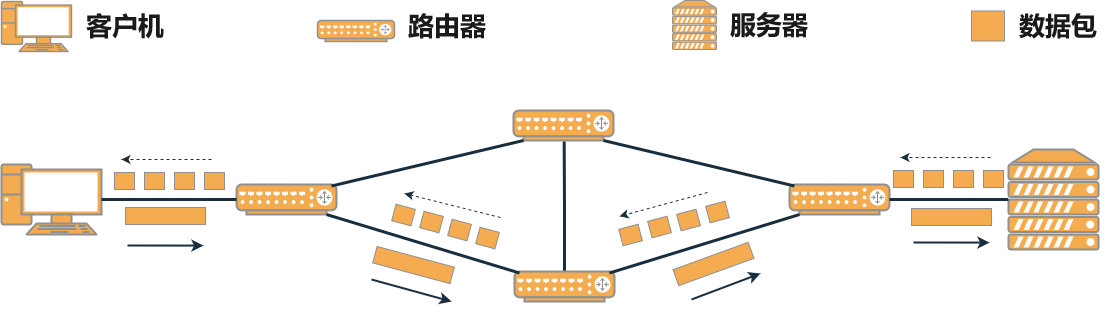
\includegraphics[width = 0.8\textwidth]{linktest.drawio.png}
%   \caption{链路测试法原理}
%   \label{fig:linktest}
% \end{figure}

% \textbf{输入调试法:}在输入调试法中每个路由器都有能力根据特定的分组特征来确定其传入的链路。受到攻击的
% 受害者可以构建一个攻击数据包签名,并将其发送到上游路由器。然后,路由器可以根据
% 接收到的攻击包签名递归地调查其上游链路,从而识别出攻击者。下面列出了这种方法的优缺点。
% \begin{itemize}
%   \item 优点:
%     \begin{itemize}
%     \item 与现有的协议和基础设施相一致。
%     \item 为增量部署提供了良好的支持。
%     \item 在网络流量上的带宽开销很小。
%   \end{itemize}
% \item 缺点:
%   \begin{itemize}
%     \item 不适合DDoS环境。
%     \item 依赖于isp之间的合作。
%     \item 跟踪系统只在攻击时运行。
%   \end{itemize}
% \end{itemize}

% \textbf{控制泛洪法:}在控制泛洪法中,受害者利用预定义的ISP地图迭代地将数据包淹没其上游路由器,
% 并同时确定攻击强度的变化。这个递归过程可以在每个上游级别上显示攻击源。下面列
% 出了这种方法的优缺点。
% \begin{itemize}
%   \item 优点:
%     \begin{itemize}
%       \item 与现有的协议和基础设施相一致。
%       \item 支持简单和增量的实现。
%     \end{itemize}
%   \item 缺点:
%     \begin{itemize}
%       \item 追踪只在持续的攻击中进行。
%       \item 需要具备网络拓扑结构的先验知识。
%       \item 对DDoS攻击无效。
%     \end{itemize}
% \end{itemize}

% \textbf{消息传递法:}消息传递在向目标传输回溯相关信息方面提供了更大的灵活性。主要采用Taylor等人
% 提出的基于互联网控制消息协议(ICMP)的方案\cite{Taylor2014ICMP}。
% 在该方案中,每个
% 路由器概率地生成一个称为跟踪包或iTrace消息的ICMP包,该包负责携带要用作回
% 溯过程的输入的信息,它可能包含下一跳和上一跳信息、
% 时间戳、MAC地址等参数。在攻击期间,成千上万个这样的iTrace数据包
% 有助于成功的回溯操作。但是,为了避免由这些消息造成的网络流量开销,消息生成的
% 概率通常会保持在可容忍的限制下。Hsu和Chiueh
% \cite{Hsu2003TrafficSourceIdentification}和Wang和Schulzrinne
% \cite{WangSchulzrinne2004DoS,WangSchulzrinne2004ReflectiveDoS}所做的工作
% 就是此类方法的代表。图~\ref{fig:messaging}~展示了消息传递法的基本原理。
% 下面列出了这种方法的优缺点。
% \begin{itemize}
%   \item 优点:
%     \begin{itemize}
%       \item 支持具有低ISP合作能力的增量部署。
%       \item 与现有的协议和基础设施相一致。
%       \item 允许对攻击后进行分析。
%     \end{itemize}
  
%   \item 缺点:
%     \begin{itemize}
%       \item 如果缺乏身份验证支持,很容易被攻击者滥用。
%       \item 由于生成额外的数据包而产生网络流量开销。
%     \end{itemize}

% \end{itemize}

% \begin{figure}[htbp]
%   \centering
%   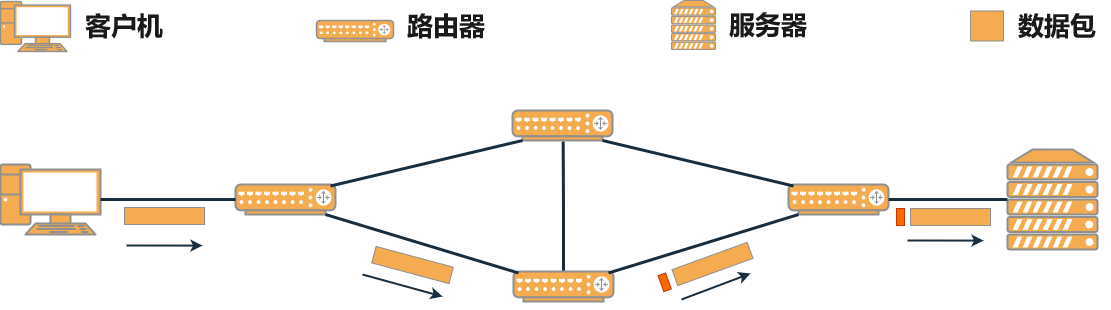
\includegraphics[width = 0.8\textwidth]{messaging.drawio.png}
%   \caption{消息传递法原理}
%   \label{fig:messaging}
% \end{figure}


% \textbf{数据包标记法:}数据包标记法背后的关键思想是利用数据包本身来记录路由信息。其原理如图~\ref{fig:packet_marking}~所示。
% 受害者使用这些信息来探索该数据包所遍历的路径。标记数据包既可以包含完整的编码路由信息,也可携带由中间路由器嵌入的
% 一个或多个标记。受害者可以识别所有收集到的标记数据包,并利用
% 存储在标记字段中的信息来跟踪攻击源。概率分组标记(PPM)和确定性分组标记
% (DPM)是两种最突出的标记方案\cite{Burch2000Tracing}。这两种方案是现有
% 文献中许多基于标记的方案的基础。~\ref{fig:ipv4_header}~展示了数据包头部字段被用来
% 填充标记信息的使用情况。
% 为避免数据包头过载以及降低路径重构过程中的误报率的需求,数据包标记法需要适当的标记编码方案,
% 此外,数据包标记法有三种主要的标记策略:节点附加法、节点采样法、边采样法\cite{Alenezi2011}。

% \begin{figure}[htbp]
%   \centering
%   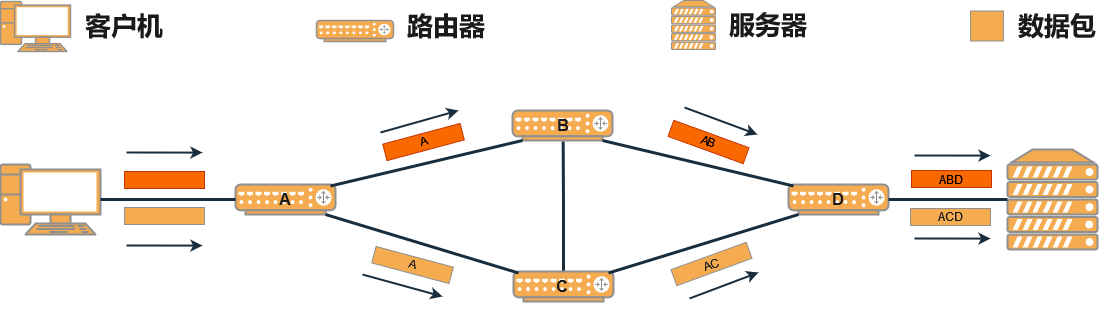
\includegraphics[width = 0.8\textwidth]{packetmarking.drawio.png}
%   \caption{数据包标记法原理}
%   \label{fig:packet_marking}
% \end{figure}

% \textbf{节点附加法:}在节点附加法中路由器的信息将会作为标记被逐个追加到原始IP包头中
% \cite{Amin2006,Min2003}。
% 这种机制通过在单个数据包中携带多个路由信息简化了标记过程。因此这种方法仅仅依靠单个标记包
% 便能确定一条完整的路径。但此种方法由于增加了过多的标记字段导致高网络带宽开销。这一缺陷也
% 限制了此种方法的应用。

% \textbf{节点采样法:}一个单个的标记数据包只会携带单个路由节点的标记信息,这就意味着当
% 路由器对将自身路由信息写入标记数据包时会覆盖掉之前的信息。不过这也导致导致标记策略的灵活
% 性降低。节点采样法的标记信息通常包括路由器的IP地址。也有许多方案为路由器分配颜色、身份
% 编号或其它特定的标记功能\cite{Jin2009,Liu2006}。

% \textbf{边采样法:}边采样法涉及到边缘信息的编码,如起始、结束等,而不是再针对单个节点
% 信息的操作。其他常见的边缘信息属性包括边缘权重、颜色、身份编号等。除了这些属性外,
% 巧妙地使用距离字段,能够让方案在不需要预先了解互联网拓扑的情况下具备构建攻击路径的能力。
% 以下列出了这种方法的优点和缺点。
% \begin{itemize}
%   \item 优点:
%   \begin{itemize}
%     \item 现有网络基础设施兼容。
%     \item 与其他方法相比,实施简单灵活。
%     \item 适用于DDoS攻击。
%     \item 需要的ISP支持最少。
%   \end{itemize}
%   \item 缺点:
%   \begin{itemize}
%     \item 由于在许多追踪方案中过载标识字段,导致数据包碎片化问题。
%     \item 有时可能产生高误报结果。
%     \item 需要修改现有协议来实现标记过程。
%     \item 追踪准确性取决于受害节点收到的标记数据包的数量。
%   \end{itemize}
% \end{itemize}




% \begin{figure}[htbp]
%   \centering
%   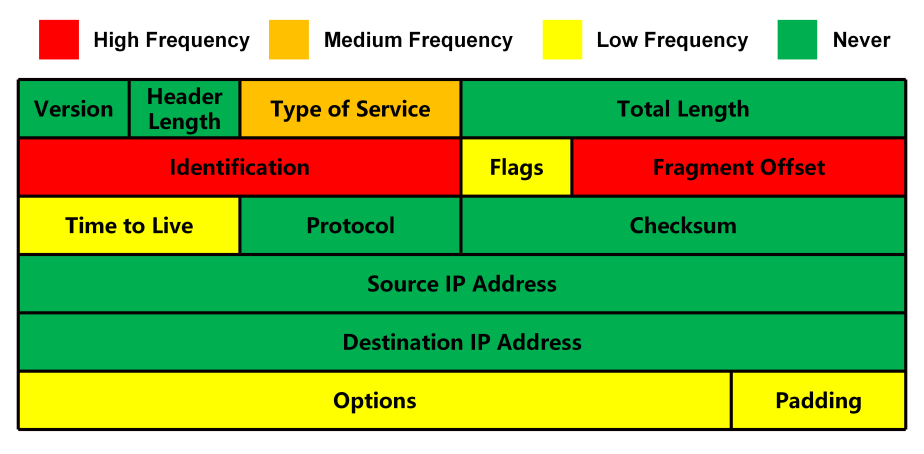
\includegraphics[width = 0.8\textwidth]{ipv4_header.png}
%   \caption{标记过程中使用的IPv4头部字段}
%   \label{fig:ipv4_header}
% \end{figure}


% \textbf{路由器日志记录法:}
% 记录法旨在将数据包摘要存储在中间路由器上。
% 然后当受害者服务器进行攻击路径重构时便可使用这些路由器上存储的信息来确定网络路径。
% 日志记录法的原理如图~\ref{fig:loggging}~所示。
% 尽管这种方法的回溯效果很不错,因为它可以使用单个数据包完成攻击路径重构,但它的一个主要缺点是:它将会给路由器带来巨大的存储开销。
% 因此,它的部署一直是一个挑战。
% Snoeren等人\cite{Snoeren2001}提出了一种基于哈希的IP追踪方法,称为源路径隔离引擎,以实际实现基于日志的IP追踪。
% 他们的方法使用了一种称为布隆过滤器的空间高效数据结构,显著减少了路由器存储数据包摘要的存储开销。
% Kai等人\cite{Kai2009}、Hilgenstieler等人\cite{Hilgenstieler2010}都对此方法提出了改进进一步增强了性能。
% 这种方法的优点和缺点如下。
% \begin{itemize}
%   \item 优点:
%   \begin{itemize}
%     \item 与协议和现有基础设施兼容。
%     \item 支持攻击后分析。
%     \item 允许追溯单个数据包。
%     \item 网络流量开销可忽略。
%   \end{itemize}
%   \item 缺点:
%     \begin{itemize}
%       \item 高内存和处理要求。
%       \item ISP合作的隐私问题对这种方法构成问题。
%       \item 需要及时进行追踪,因为路由器会定期刷新以前记录的信息。
%     \end{itemize}
% \end{itemize}

% \begin{figure}[htbp]
%   \centering
%   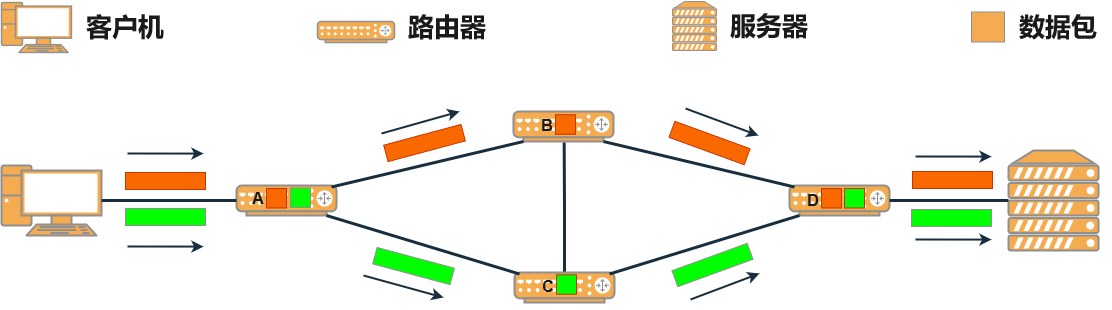
\includegraphics[width = 0.8\textwidth]{logging.drawio.png}
%   \caption{路由器日志记录法原理}
%   \label{fig:loggging}
% \end{figure}

% \textbf{覆盖法:}一个覆盖网络主要由用来跟踪路由的专用路由器组成,这些专用路由器被称为跟踪路由器。
% 这些路由器的主要职责是监控流量,当检测到攻击时,覆盖网络将发出命令指示流量通过这些专用路由器。
% 然后,这些路由器检查通过它们的流量,并提取用于追踪来源的信息。图~\ref{fig:overlay}~Stone提出了这样一个系统,称为CenterTrack,它通过分析通过中心化跟踪路由器的流量来提供追踪服务\cite{stone2000centertrack}。
% Castelucio等人\cite{castelucio2009aslevel}和Tian等人\cite{tian2011easytrace}提出的工作也采用了基于覆盖的方法进行IP追踪。这种方法的优点和缺点如下。
% \begin{itemize}
%   \item 优点:
%   \begin{itemize}
%     \item 提供准确的追踪结果。
%     \item 有效处理DDoS攻击。
%     \item 客户端免于执行追踪过程。
%   \end{itemize}

  
%   \item 缺点:
%   \begin{itemize}
%     \item 实施成本高。
%     \item 缺乏对渐进式部署的支持。
%     \item 跟踪路由器本身可能成为DDoS攻击的目标。 
%   \end{itemize}

% \end{itemize}

% \begin{figure}[htbp]
%   \centering
%   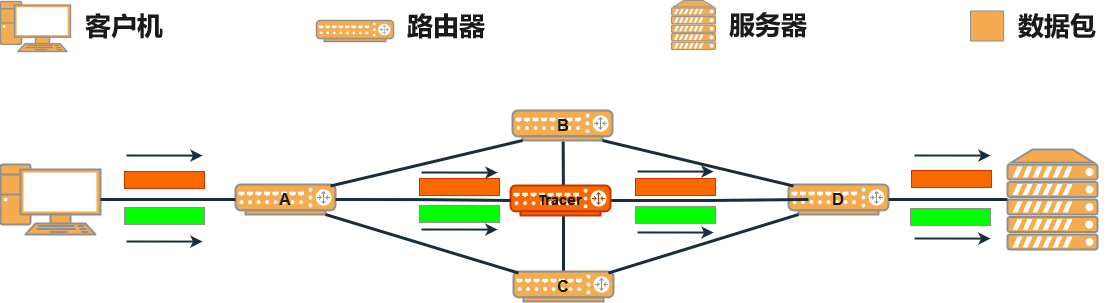
\includegraphics[width = 0.8\textwidth]{overlay.drawio.png}
%   \caption{覆盖法原理}
%   \label{fig:overlay}
% \end{figure}

% \textbf{模式分析法:}在攻击进行时,路由器可以提取流量模式信息,这些信息可以用于溯源,如Xiaofeng等人\cite{xiaofeng2004mechanism}、
% Chen等人\cite{chen2006tracing}和Lai等人\cite{lai2008antbased}所提出的。在这种方法中所有参与溯源的路由器以分布式方式相互合作,收集流量信息并追踪攻击源。
% 这使得受害者免于执行追踪任务,这被认为是这种方法的一个主要优点。
% 这种方法的优点和缺点如下。
% \begin{itemize}
%   \item 优点:
%     \begin{itemize}
%       \item 客户端免于执行追踪过程。
%       \item 追踪过程的分布式处理。
%       \item 提供了改善的可扩展性。
%     \end{itemize}
%   \item 缺点:
%     \begin{itemize}
%       \item 由于持续的流量监控,路由器处理开销大。
%       \item 在DDoS攻击中,随着攻击流量的增加,复杂性增加。
%     \end{itemize}
% \end{itemize}

% \begin{table}[htbp]
%   \caption{IP回溯方法性能比较}
%   \label{tb:compare_approch}
%   \centering
%   \begin{tabular}{ccccccc}
%   \toprule
%   {\heiti 回溯方法} & {\heiti 管理开销} & {\heiti 网络开销} & {\heiti 路由器开销} & {\heiti ISP合作} & {\heiti 假阳率} & {\heiti 时间开销}\\
%   \midrule
%   链路测试法 & Moderate &  Low & Moderate & Collaborative & High & Long\\
%   数据包标记法 & Low & Low & Low & Noncollaborative & Low & Long\\
%   路由器日志记录法 & High & Low & High & Collaborative & Low & Middle\\
%   消息传递法 & Low & Low & Low & Noncollaborative & Very Low & Long\\
%   覆盖法 & Low & Low & High & Collaborative & Low & Middle\\
%   模式分析法 & Low & Moderate & High & Collaborative & Low & Middle\\
%   \bottomrule
%   \end{tabular}
%   \end{table}


% \subsection{网络攻击检测研究现状}
异常流量检测的研究主要可以分为基于传统机器学习方法和基于深度学习的方法。\par
1)基于机器学习的方法\par
在18世纪50年代,机器学习技术还处于其早期探索阶段,标志性事件之一是1952年亚瑟·萨缪尔开发的能够在IBM 701上运行的西洋跳棋程序,这是机器学习应用的早期例证。
进入60年代,随着最近邻算法(Nearest Neighbor Algorithm)\cite{cover1967nearest}的提出,模式识别和机器学习技术开始取得初步发展。
随后的几十年见证了机器学习技术的快速成熟,诸如决策树\cite{Quinlan1986}、支持向量机(SVM)\cite{Cortes1995}、随机森林\cite{Breiman2001}等算法相继被提出。
这些算法的发展不仅推动了机器学习领域的进步,也为后来的攻击检测技术打下了坚实的基础。
特别是,支持向量机(SVM)和随机森林等算法开始被集成到入侵检测系统中,标志着基于机器学习方法的网络攻击检测技术的蓬勃发展\cite{Mukkamala2002}。
这些基于机器学习的攻击检测技术,具体可分为有监督学习和无监督学习。



有监督的机器学习攻击检测技术主要依赖于预先标记的数据集来训练模型,使其能够识别和区分正常行为与恶意行为。
这种技术通常涉及将数据集分为训练集和测试集,其中训练集用于训练模型,而测试集则用于评估模型的性能。
有监督学习的关键在于拥有大量已经被标记为正常或攻击的样本,这些样本用于让机器学习算法“学习”识别攻击行为的模式。
在有监督的机器学习攻击检测领域,主要可以分为以下几种类型:基于异常的检测、基于签名的检测、以及基于行为的检测。
每种类型都有其独特的方法和应用场景。


基于异常的检测技术通常依赖于机器学习模型来识别与已知正常行为模式显著偏离的行为。
早期的工作可以追溯到1990年代,其中Lee和Stolfo等人\cite{lee1998dataMining}在1998年的研究中对异常检测技术做出了重要贡献,提出了使用数据挖掘技术来识别网络入侵的方法。
之后Schonlau等人在2001年提出的MASQUE模型,旨在通过监视用户行为来检测异常,进而识别潜在的攻击活动。

基于签名的检测技术则是基于已知攻击的特定模式或签名来识别攻击。
这种方法的关键在于建立一个广泛的攻击特征库。
Kumar和Spafford\cite{kumar1994adep}在1994年的研究中,通过他们的工作ADEPTS,为基于签名的检测技术做出了显著贡献,发展了一种基于异常检测和签名匹配的混合方法来提高检测的准确性。

基于行为的检测技术关注于分析系统或网络中的行为模式,以识别潜在的恶意活动。
这种方式侧重于学习和理解系统或用户的正常行为模式,以便任何偏离这些模式的行为都可能被标记为恶意的。
在这个方向上,Anderson等人\cite{anderson1995userBehavior}在1995年提出了一种基于用户行为分析的入侵检测系统,该系统通过学习正常的用户行为模式来识别异常活动。
这种类型的研究在2000年代初期得到了加强,其中Forrest等人\cite{forrest1996selfImmune}在自身免疫系统的概念上的工作为基于行为的检测提供了理论基础,推动了基于行为的检测技术的发展。



无监督的机器学习攻击检测技术不依赖于预先标记的数据集,而是通过分析数据中的模式、异常或者关系来识别可能的恶意行为。
这种技术尤其适用于那些标签数据稀缺或者完全没有标签的情况,允许模型自行发现数据集中的结构。
在无监督学习领域,主要的攻击检测方法包括聚类、异常检测以及密度估计等。

聚类是一种常见的无监督学习技术,通过将数据分成由相似对象组成的多个组来工作。
在攻击检测中,聚类方法可以用来识别出不寻常的数据点集合,这些集合可能代表了恶意活动。
Portnoy等人\cite{portnoy2001clustering}在2001年的研究中通过聚类技术成功识别出异常行为,展示了聚类方法在入侵检测中的有效性。

异常检测技术在无监督学习中也占有一席之地,与有监督学习中的基于异常的检测技术相似,但不依赖于预标记的数据。
Eskin等人\cite{eskin2002anomaly}在2002年的工作中提出了一种基于异常检测的入侵检测系统,该系统能够在没有任何先验知识的情况下识别攻击行为。

密度估计方法,如局部异常因子(LOF)算法,通过评估数据点在其邻域的密度来识别异常点。
这种方法适用于发现那些在低密度区域的数据点,可能指示着异常或攻击行为。
Schubert等人\cite{schubert2014local}在2014年对LOF算法进行了改进,以增强其在检测网络入侵方面的性能。

虽然传统机器学习方法在处理一些简单的异常流量检测问题上相对方便,但在应对复杂、非结构化以及高维度流量特征数据时很难有效地学习到深层次的特征。
因此,越来越多的研究人员开始采用深度学习方法,以提高网络异常流量检测的效率和准确性。\par

2) 基于深度学习的方法\par
深度学习是机器学习的一个分支,它通过使用具有多个隐藏层的神经网络来模拟人类大脑的工作方式,从而解决复杂的模式识别问题。
1943年,McCulloch和Pitts提出了最早的神经网络模型。
1986年,Rumelhart, Hinton和Williams重新引入了反向传播算法,使得训练多层神经网络成为可能。
2006年,Hinton和他的学生提出了深度置信网络,标志着深度学习的复兴。
随后,在2010年代初,随着深度学习技术的发展,研究人员开始探索其在网络安全和攻击检测中的应用。
深度学习在处理和分析大规模复杂数据方面的能力,使其成为提高攻击检测性能的有力工具。

基于深度学习的攻击检测技术,根据其学习和推理的方式,可以大致分为生成式方法、判别式方法和混合式方法。


生成式方法旨在学习数据的联合分布$P(X,Y)$,其中$X$是输入数据,$Y$是标签。
这种方法通过模拟数据生成过程来理解和识别正常与异常模式。
在攻击检测中,生成式模型可以用于生成与真实数据分布相似的样本,从而帮助识别潜在的攻击行为。
典型的生成式模型包括深度信念网络(DBNs)和生成对抗网络(GANs)。
2014年,Goodfellow等人提出了生成对抗网络(GANs)\cite{goodfellow2014generative},这是一种强大的生成式模型,能够生成与真实数据几乎无法区分的数据样本。
在攻击检测领域,GANs被用于生成攻击数据,以帮助训练模型更好地识别和适应新的攻击类型。
2015年,An和Cho探索了使用变分自编码器(VAE)进行异常检测的方法\cite{an2015variational}。
该方法通过计算输入数据的重构概率来识别异常,展示了VAE在复杂数据集上进行无监督异常检测的潜力。


判别式方法专注于学习从输入数据到标签的条件概率分布$P(Y∣X)$。
这类方法通过区分不同类别的数据特征来进行分类或预测。
在攻击检测应用中,判别式模型,如卷积神经网络(CNNs)和循环神经网络(RNNs),被广泛用于直接识别各种类型的网络攻击,因为它们能够有效处理和分析大量的网络数据。
2015年,Saxe和Berlin展示了如何使用深度CNN来检测恶意软件\cite{saxe2015deep}。
他们通过将二进制文件转换为二维图像,然后使用CNN进行特征学习和分类,有效提高了恶意软件检测的准确率。
2019年,在论文中\onlinecite{staudemeyer2019applying},Staudemeyer和Morris展示了如何利用LSTM网络来检测DDoS攻击。
他们利用RNN的时间序列学习能力,有效识别了网络流量中的异常模式。

混合式方法结合了生成式和判别式方法的优点,以提高模型的泛化能力和准确性。
这种方法通常涉及使用生成模型来增强数据或特征,随后通过判别模型进行精确的分类或检测。
混合式方法在攻击检测中特别有用,因为它们可以通过生成式组件来理解和模拟攻击行为的复杂性,同时利用判别式组件的强大分类能力来准确识别攻击。
2018年,Li及其团队提出了MAD-GAN\cite{li2018mad},一种结合生成对抗网络和深度学习模型的方法来检测时间序列数据中的多变量异常。
这种方法通过GAN生成的模拟异常数据来训练深度学习模型,从而提高了模型对新型攻击行为的检测能力。
2019年,Feng及其团队提出了一种结合自编码器和卷积神经网络的方法来检测物联网(IoT)网络中的异常行为\cite{feng2019deep}。
该方法首先利用自编码器学习正常网络流量的特征表示,然后使用CNN对流量进行分类,有效识别了异常模式。


\section{论文研究内容}
% 在众多的网络回溯方法中,数据包标记法与其他方法相比具有简单、灵活、易于部署、无需人工参与、支持事后分析等优点,但此类方法仍然存在一些局限性和改进的空间。
% 在PPM方案中,完成路径覆盖进行路径重构所需要的数据包数量与受害者服务器到攻击者主机的距离d成指数关系。
% 因此当d特别大时,路径重构的过程是十分缓慢的。DPM方案虽然可以弥补PPM存在的缺陷,但此方案需要将整条路径上的路由信息(通常为IP地址)追加到数据包头部,这将会导致IP包头过大而带来一系列问题。
% 因此本文首先综合考虑两种方案的优缺点,巧妙地利用路由器接口号的局部性,设计一种改进的数据包标记方案,在不扩大数据包头部的情况下在单个数据包上对多个路由器进行标记成为可能。\par

% 尽管当今网络攻击检测技术已取得了显著进步,但仍存在诸多不足。
% 首先,当今的检测模型通常只关注流量数据的单一维度特征,当面对维度不断攀升的流量数据时,无法充分应对日益复杂的网络攻击,模型的检测能力将会有所下降。
% 针对上述问题,本文提出了一种基于残差网络与双向门控循环单元的多模态特征融合模型。
% 该模型不仅能够深入挖掘数据中的空间特征与时序特征,还能通过综合分析这些特征,做出更为精准的决策。

% 另外,当前检测技术多依赖于静态数据集,难以适应快速变化的网络环境,导致在实际应用中面临诸多挑战。
% 为了应对不断变化的网络环境,本文引入了iCaRL()技术\cite{},使本文所提的模型进在保留对原有知识的基础上实现对新攻击模式的快速学习和适应,从而确保网络安全的持续性和稳定性。
% 最后为了使我们的模型当面对DDoS攻击时能够正常运作并从源头上解决DDoS攻击,本文将为模型提供一套防护技术,当时别到攻击流量后可针对流量进行具体的溯源从源头上对其进行处置。

尽管现有的网络攻击检测技术已经取得了长足的进步,但在实际应用中仍然暴露出不少短板。
首要问题在于,现有的检测模型大多仅聚焦于流量数据的单一维度特征,这在面对日益复杂且多维度的流量数据时显得力不从心,导致模型的检测效能大打折扣。
为了弥补这一不足,本文提出了一种基于残差网络与双向门控循环单元的多模态特征融合模型。
这一模型不仅能够有效挖掘数据中的空间与时序特征,更能通过全面、综合的分析,做出更为精准的判断,从而显著提升检测的准确性和可靠性。
此外,当前的网络攻击检测技术多依赖于静态数据集,这在快速变化的网络环境中显得捉襟见肘,实际应用中面临诸多挑战。
为了应对这一挑战,本文引入了iCaRL技术并基于遗传算法对该技术进行了优化改进,使得所提模型能够在保留原有知识的基础上,迅速学习并适应新的攻击模式,确保网络安全的持续性和稳定性。
最后,为了确保模型在面对DDoS攻击时能够稳定运行,并从根本上解决问题,本文还将为模型设计一套专门的防护技术。
一旦模型识别到攻击流量,我们将为其配备一套专门的机制,能够迅速定位并处理异常流量,从源头上消除威胁,确保模型的稳定运行。
% 其次,尽管机器学习和深度学习技术已广泛应用于网络异常流量检测,但挑战仍然存在,特别是在准确性和未标记数据处理方面的局限性凸显了现有方法的不足。
% 因此,为了能够处理少量标记数据的情况和达到更高的检测精度,以及能够有效挖掘复杂网络数据的深层特征,我们引入了基于遗传算法和增量学习提升的ResNet-BiGRU混合模型。
% 最后,考虑到网络环境中常见的问题,即在运行过程中往往忽略了对数据包源地址真实性的验证,导致攻击者可能利用伪造的IP地址发起攻击。
% 为此,本文会将提出的攻击检测方法与溯源技术相结合,开发一套网络攻击检测及溯源系统。
% 该系统旨在不仅能够准确检测出网络攻击行为,而且能进一步追踪到发起攻击的主机的真实位置,有效应对攻击者使用伪造IP地址的策略。
因此,本文的研究内容及主要贡献如下:\par

1)鉴于当前网络攻击检测技术主要关注流量数据的单一维度,特征挖掘不足,导致异常流量检测精准度有待提升。
为此,本文创新性地提出了一种基于残差网络与双向门控循环单元的多模态特征融合模型。
该模型结合残差网络的强大空间特征提取能力与双向门控循环单元的时序特征分析优势,通过多模态特征融合技术,全面深入地分析流量数据的时空特征,进而提升检测精准度。\par

2)针对当前的网络攻击检测技术大多依赖于静态的数据集,难以适应快速变化的网络环境的问题,
本文引入了iCaRL技术并基于遗传算法对该技术进行了优化改进,使得所提模型能够在保留原有知识的基础上,迅速学习并适应新的攻击模式,确保网络安全的持续性和稳定性。\par

3)为应对DDoS攻击对模型可能造成的严重负担,本文基于数据包标记溯源原理,创新性地设计并提出了一种基于路由器接口号分组的概率标记溯源方法——IGPPM。
该方法充分利用路由器接口号的局部性特点,在不增加数据包大小的情况下,对路径上的一组连续路由器进行有效标记。    d              
这使得单个数据包能够携带更为丰富的路由信息,从而迅速且准确地完成路径溯源工作。
一旦定位到攻击者源头,便能从源头处直接过滤掉攻击流量,有效减轻模型的负担,确保网络的安全稳定。\par

% 该模型充分融合了残差网络在特征提取方面的优势与双向门控循环单元在处理时序数据时的长处,从而实现对流量数据时空特征的深度挖掘。
% 通过综合分析这些特征,模型能够做出更为精准的攻击检测决策。
% 在UNSW-NB15数据集上的实验结果表明,相较于传统机器学习模型以及ResNet、BiGRU等模型,本模型在准确率方面表现出色,为攻击检测任务提供了更加高效和可靠的解决方案。\par



\section{论文组织结构}
本论文一共有5个章节,其组织结构如图~\ref{fig:paper_structure}~所示。
\begin{figure}[htbp]
  \centering
  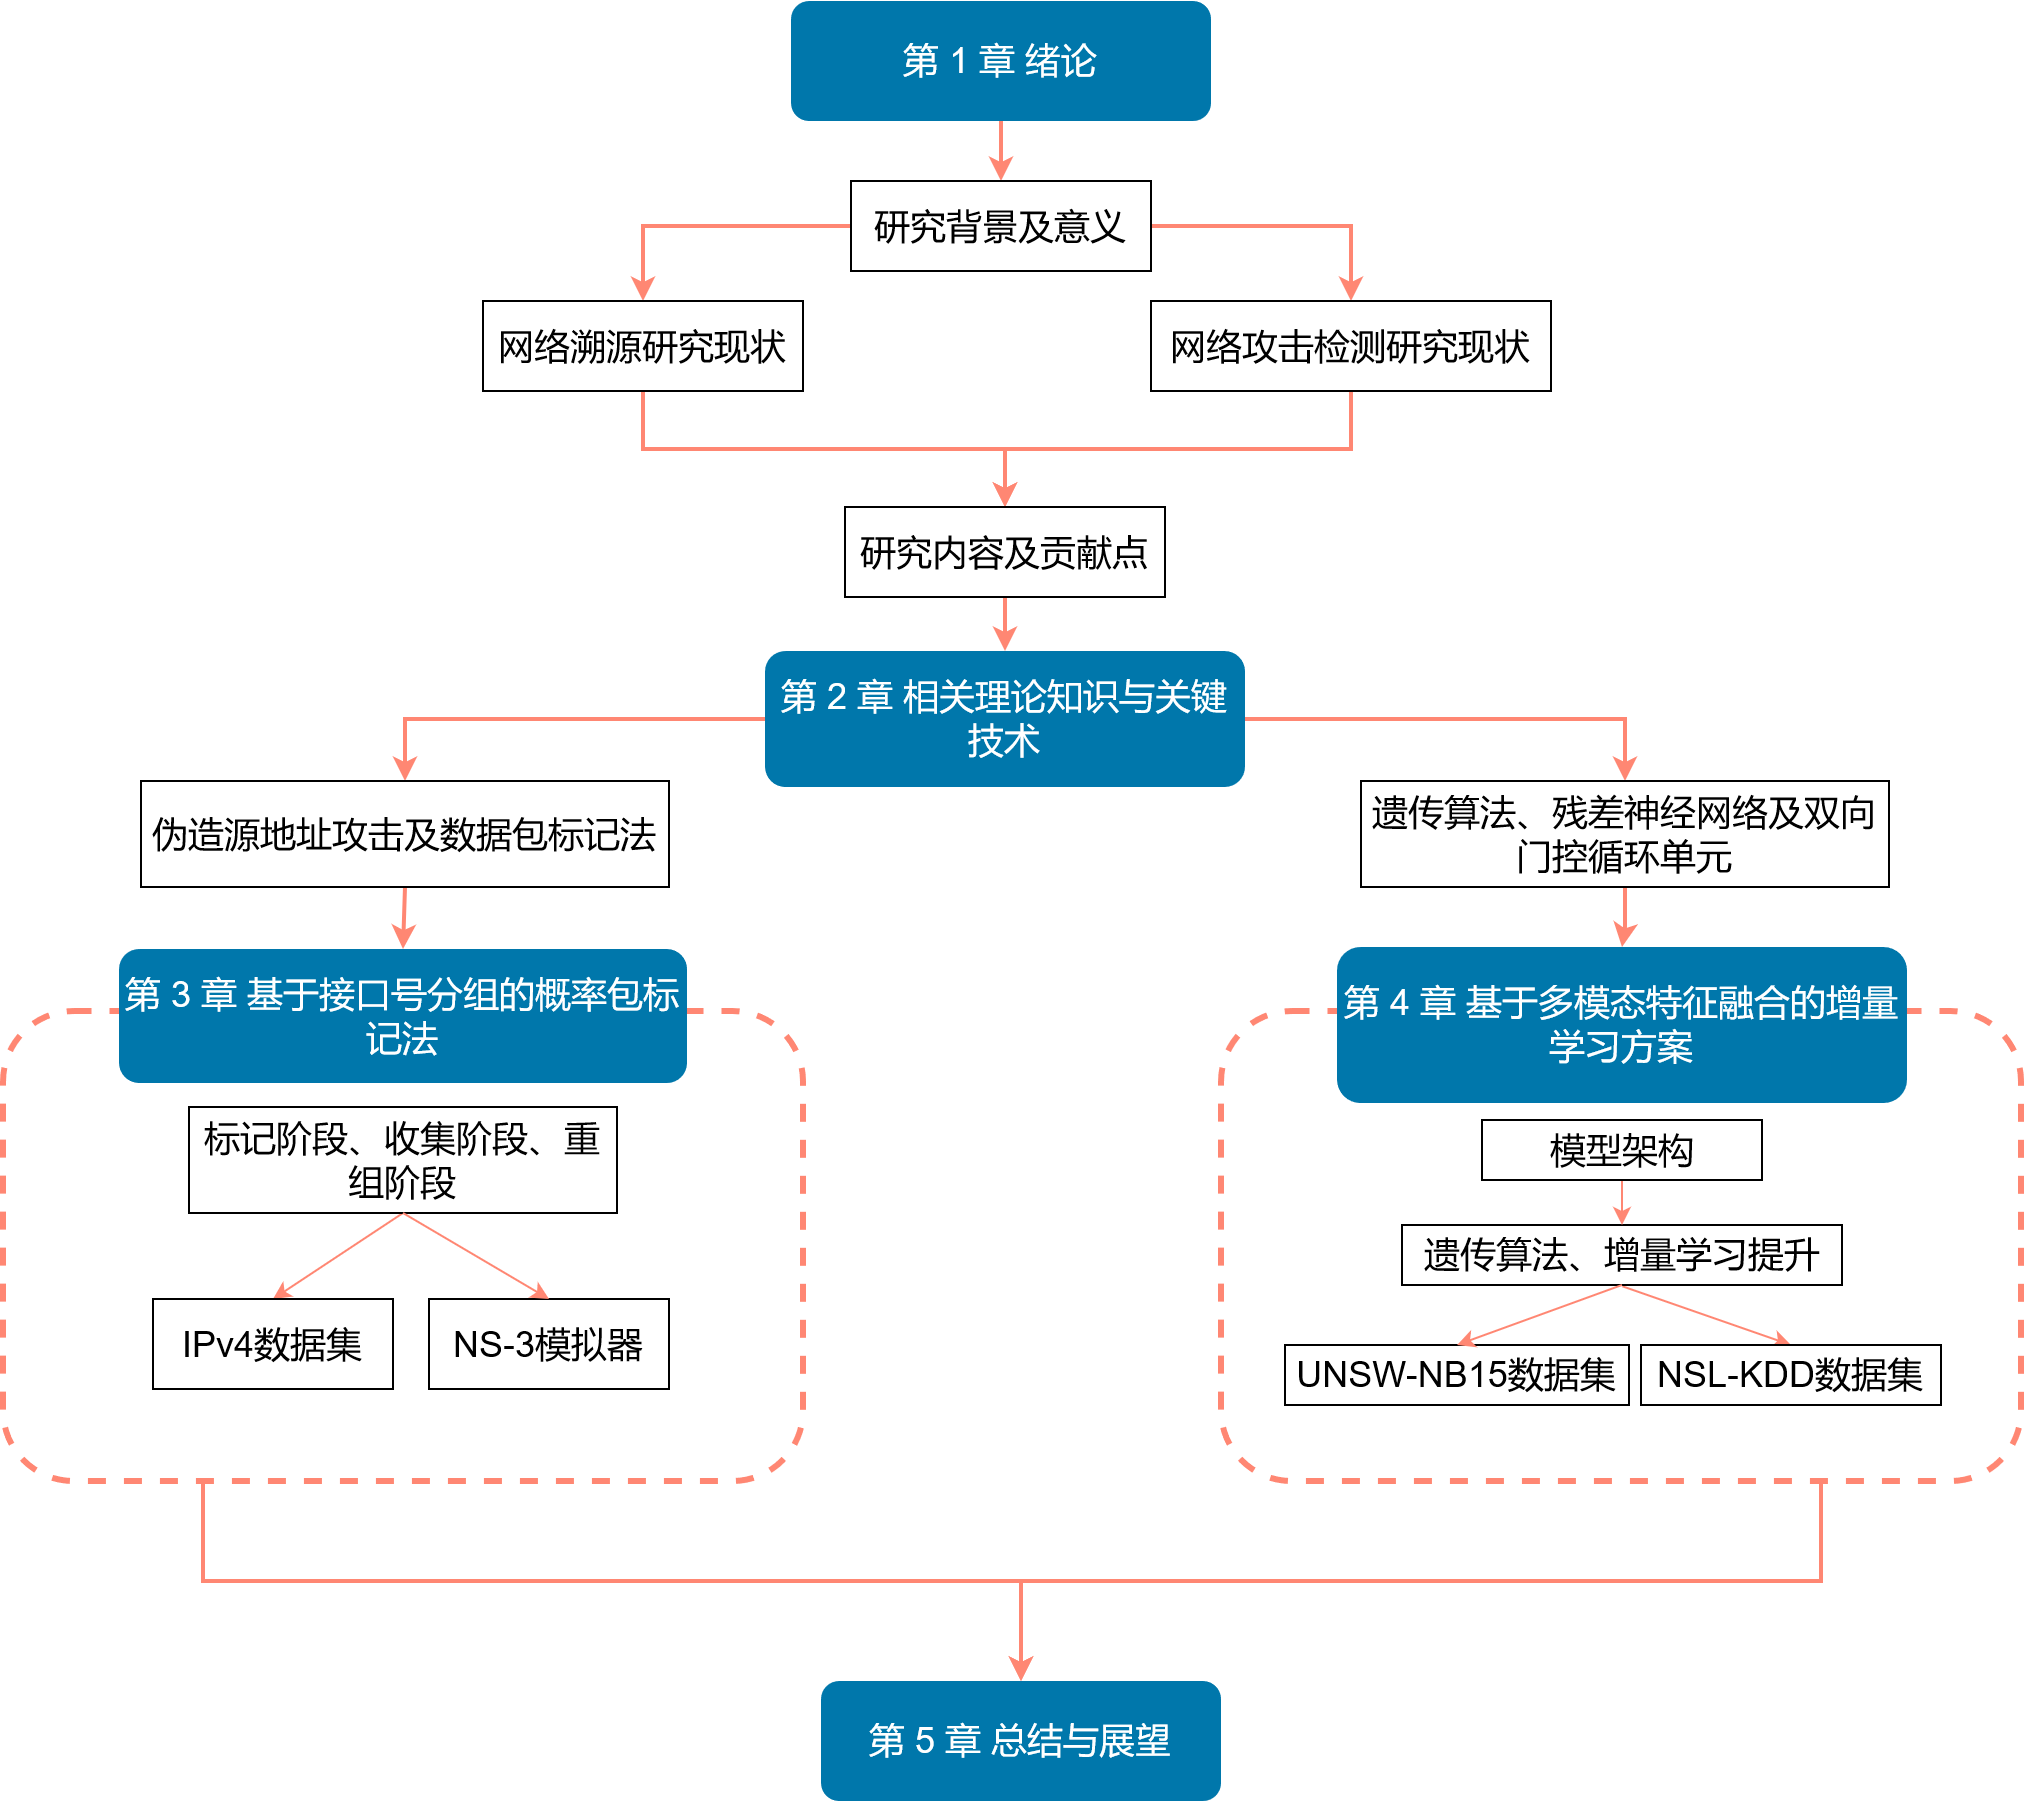
\includegraphics[width = 0.8\textwidth]{paper_structure.drawio.png}
  \caption{论文组织结构}
  \label{fig:paper_structure}
\end{figure}

第~\ref{cha:overview}~章,绪论。
在本章主要介绍了我们的研究,即基于特征融合的异常流量检测模型及防护方法研究,所处的背景以及具备的研究意义。
之后,本文详细地介绍了网络溯源技术的研究现状。
最后交代了本文的研究内容及主要贡献点以及论文的组织架构。


第~\ref{cha:basic-knowledge}~章概述了残差神经网络、双向门控循环单元网络、遗传算法、伪造源地址攻击与数据包标记法的相关理论基础。

% 第~\ref{cha:ResNet-BiGRU}~章, 基于特征融合的异常流量检测模型与增量学习实现。
% 本文首先提出了一个基于残差网络与双向门控循环单元的多模态特征融合模型,并对其原理和结构进行了详细的介绍。
% 随后经过几组对比实验验证了该模型的优越性。
% 接着,本文又基于此模型结合iCaRL技术提出了一个多模态特征融合的增量学习方案。
% 为进一步优化该方案的性能,本文又提出了一个基于遗传算法的记忆集抽样优化策略。
% 最后利用UNSW-NB15和NSL-KDD数据集分别作为新旧任务数据集对该方案进行了验证,验证结果表明该方案能够有效支持模型的增量学习和知识保留。


第~\ref{cha:ResNet-BiGRU}~章首先提出了基于残差网络与双向门控循环单元的多模态特征融合模型,并通过实验验证了其优越性。
接着本文基于此模型结合iCaRL技术,实现了增量学习方案。
为进一步优化该方案的性能,本文又提出了一个基于遗传算法的记忆集抽样优化策略。
最后利用UNSW-NB15和NSL-KDD数据集分别作为新旧任务数据集对该方案进行了实验验证,实验证明该方案能有效支持模型增量学习和知识保留。

第~\ref{cha:IGPPM}~章,基于接口号分组的概率标记溯源防护方法。
本章首先提出了基于接口号分组的概率标记溯源防护方法,并介绍了该方法的原理及流程。
随后,本文通过几组对比实验,展示了该溯源方法在溯源准确率和溯源速度方面的性能表现。
最后,本文设计了该溯源方法对模型进行防护的具体原理和流程。

% 第~\ref{cha:IGPPM}~章提出了基于接口号分组的概率标记溯源防护方法,包括其运行的三个阶段。
% 通过对比实验,展示了该方法在溯源准确率和速度上的优势,最后详细设计了其对模型保护的原理和流程。


第~\ref{cha:over_view}章,总结和展望。
总结了本文的所有研究工作以及取得的成果,最后指出了本文未来的研究内容和方向。

最后是参考文献、攻读硕士学位期间发表的学术论文目录和致谢。
